\section{System Design}

\subsection{Functional Requirements}
The Student Life Support Service is designed to fulfill the specific functional requirements of three key user roles: Students, Dormitory Staff (or Student Affairs), and Administrators. Each role has its own set of features tailored to its needs within the system.

\noindent \textbf{User Type}: S-Student, DS-Dormitory Staff/Student Affairs, A-Admin (Operator) \\
\textbf{Categorized}: F-Functional, NF-Nonfunctional

\newcolumntype{L}{>{\arraybackslash}m{3.5cm}}
\begin{longtable}{|m{0.6cm}|m{2.8cm}|m{5.4cm}|m{1.6cm}|m{1.5cm}|m{1.8cm}|}
	\hline
	\textbf{No} & \textbf{Requirement }             & \textbf{Description}                                                                                          & \textbf{Priority} & \textbf{User Type}  & \textbf{Category} \\ \hline
	\endhead
	1  & Manage personal info     & Users can view and update their personal information.                                                 & Medium   & S, DS, A   & F           \\ \hline
	2  & Support tickets          & Users can create (raise), view support tickets.                                                       & High     & S, DS, A   & F           \\ \hline
	3  & Contact through messages & Users can contact the staff or students handling the support ticket through text messages.            & High     & S, DS      & F           \\ \hline
	4  & Ticket rating            & Students can rate their tickets which are marked as done.                                             & Medium   & S          & F           \\ \hline
	5  & View newsfeed            & Users can view a newsfeed of public pending/in-process tickets.                                        & Low      & S, DS, A   & F           \\ \hline
	6  & View notifications       & Users can view notifications and announcements.                                                       & Medium   & S, DS, A   & F           \\ \hline
	7  & Feedback and suggestions & Users can give feedback and suggestions for the system.                                                & Medium   & S, DS, A   & F          \\ \hline
	8  & Handle support tickets   & Dormitory staff can view and handle (mark as done, cancel) support tickets.                            & High     & DS         & F           \\ \hline
	9  & View past tickets        & Dormitory staff can view all previously handled support tickets.                                       & Medium   & DS         & F           \\ \hline
	10 & Manage notifications     & Dormitory staff and admins can create and manage notifications and announcements.                      & High     & DS, A      & F           \\ \hline
	11 & Manage users             & Admins can manage all users/roles (create, view, update, delete).                                      & High     & A          & F           \\ \hline
	12 & Manage tickets           & Admins can manage all support tickets (view, delete).                                                  & High     & A          & F           \\ \hline
	13 & Manage dormitories       & Admins can manage all dormitories (create, view, delete).                                              & Medium   & A          & F           \\ \hline
	14 & Manage system logs       & Admins can manage system logs (view, delete).                                                          & Medium   & A          & F           \\ \hline
	15 & Manage feedback          & Admins can manage system feedback (view, delete).                                                      & Low      & A          & F           \\ \hline
	16 & View system report       & Admins can generate and view system reports.                                                           & High     & A          & F           \\ \hline
	
	
	\caption{Functional Requirements}
	\label{tab:functionalRequirement}
\end{longtable}


For clearer comprehension, the table presented below provides a detailed visualization of the functional requirements, organized according to the different user roles within the system. This structure allows for a more precise understanding of how each role interacts with the system's features and capabilities.

\begin{longtable}{{|m{4.8cm}|m{12cm}|}} 
	\hline
	\textbf{User roles} & \textbf{Functional Requirements}\\ \hline
	\endhead
	
	Student & 	
	\begin{itemize}
		\item can view, update his/her personal information.
		\item can create (raise), view his/her support tickets. 
		\item can contact the staff who handles the support ticket through text messages.
		\item can rate his/her tickets which are marked as done.
		\item can view newsfeed (public pending/in process tickets).
		\item can view notifications, announcement.
		\item can give feedback and suggestions for the system.
	\end{itemize}
	
	\\ \hline
	
	Dormitory staff/ Student Affairs & 	
	\begin{itemize}
		\item can view, update his/her personal information.
		\item can view all available support tickets.
		\item can handle support tickets. (mark as done, cancelled)
		\item can view all past handled tickets.
		\item can contact students who owns the ticket through text messages.
		\item can view newsfeed (public pending/in process tickets).
		\item can create, view notifications, announcement. 
		\item can give feedback and suggestions for the system.
	\end{itemize}
	
	\\ \hline
	
	
	Admin (Operator) & 	
	\begin{itemize}
		\item can manage his/her personal information (view, update).
		\item can manage all users/roles (create, view, update, delete).
		\item can manage all support tickets (view, delete).
		\item can manage all dormitories (create, view, delete).
		\item can manage system logs (view, delete).
		\item can manage system feedback (view, delete).
		\item can view newsfeed (public pending/in process tickets).
		\item can manage notifications, announcement (create, view). 
		\item can view the system report.
	\end{itemize}
	
	\\ \hline
	
	
	\caption{Functional Requirements by User Roles} % needs to go inside longtable environment
	\label{tab:functionalRequirements}
\end{longtable}



\subsection{Non-Functional Requirements}
\noindent \textbf{Categorized}: NF-Nonfunctional

\newcolumntype{L}{>{\arraybackslash}m{3.5cm}}



	\begin{longtable}{|m{0.5cm}|m{2.5cm}|m{7cm}|m{1.5cm}|m{1.7cm}|m{2.4cm}|}
		\hline
		\textbf{No} & \textbf{Requirement}                & \textbf{Description}                                                                                                                               & \textbf{Priority} & \textbf{Category}  & \textbf{Functioning} \\ \hline
		\endhead
		1  & Fast Response Time          & The system should provide fast responses for user interactions such as submitting tickets, viewing statuses, and real-time messaging.      & High     & NF        & Performance \\ \hline
		2  & Real-Time Communication     & Messages between students and staff should be transmitted with minimal latency (under 100 milliseconds).                                   & High     & NF        & Performance \\ \hline
		3  & Concurrent Users            & The system must support up to 500 concurrent users without significant performance degradation.                                            & High     & NF        & Performance \\ \hline
		4  & Database Query Optimization & PostgreSQL database should be optimized to handle high read/write volume efficiently even during peak load.                                & High     & NF        & Performance \\ \hline
		5  & JWT-Based Authentication    & Secure authentication using JSON Web Tokens (JWT), with short-lived tokens and securely stored refresh tokens in Redis.                    & High     & NF        & Security    \\ \hline
		6  & Role-Based Access Control   & Enforce strict role-based access to ensure users only have access to the functionality appropriate for their role.                         & High     & NF        & Security    \\ \hline
		7  & Encryption                  & All communications between the client and server must be encrypted using HTTPS to ensure data security.                                    & High     & NF        & Security    \\ \hline
		8  & Data Validation             & Input from users must be validated and sanitized to protect against common vulnerabilities like SQL Injection and Cross-Site Scripting.     & High     & NF        & Security    \\ \hline
		9  & Audit Logs                  & Admins must have access to immutable and secure audit logs to track user actions such as login attempts and system modifications.           & Medium   & NF        & Security    \\ \hline
		10 & Database Scalability        & The PostgreSQL database should scale efficiently as the number of tickets, messages, and users grows.                                       & High     & NF        & Scalability \\ \hline
		11 & User-Friendly Interface     & The interface should be intuitive and easy to navigate for users of varying technical abilities.                                            & High     & NF        & Usability   \\ \hline
		12 & Cross-Device Compatibility  & The system should be responsive and function well on desktops, laptops, tablets, and smartphones.                                           & High     & NF        & Usability   \\ \hline
	
		\caption{Non-Functional Requirements}
	\label{tab:nonfunctionalRequirements}
	
	\end{longtable}



\subsection{Use Case Diagrams}
	\begin{figure}[H]
		\centering
		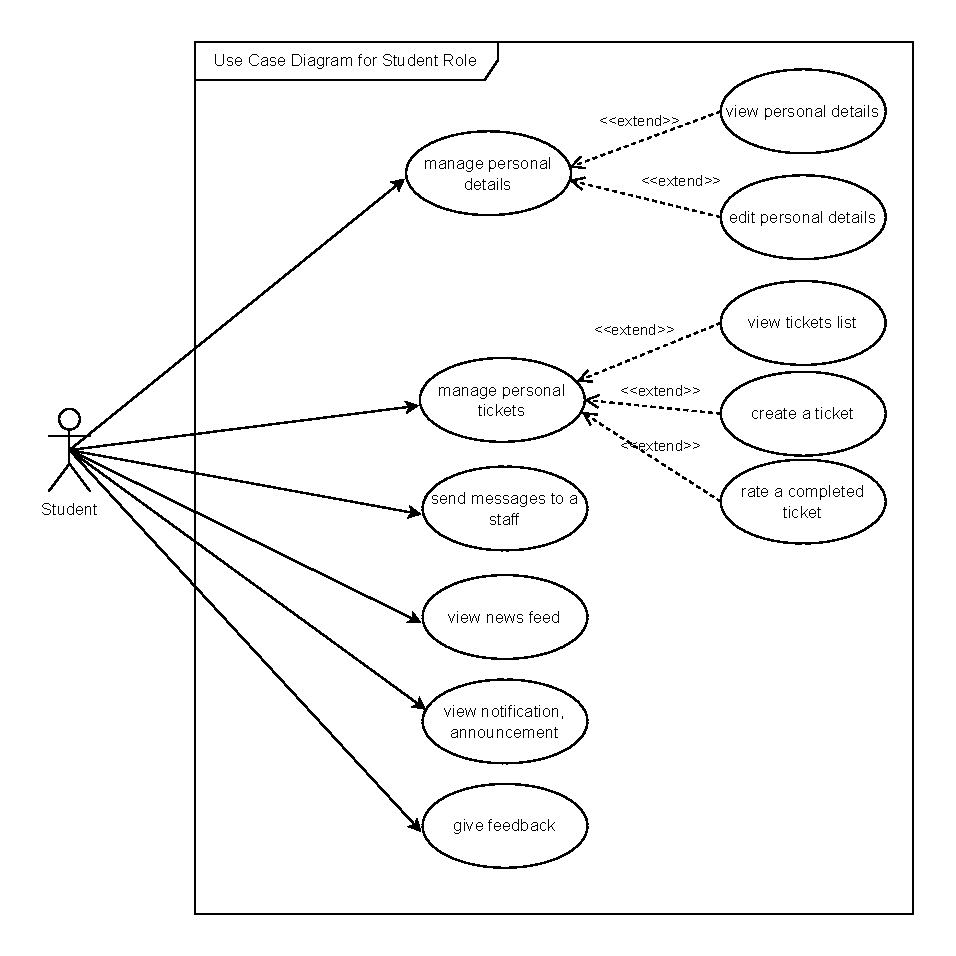
\includegraphics[width=0.82\columnwidth]{graphics/student use case.pdf}
		\caption{Student Use Case Diagram}
		\label{fig:student-use-case}
	\end{figure}
	
	
	
	\begin{figure}[H]
		\centering
		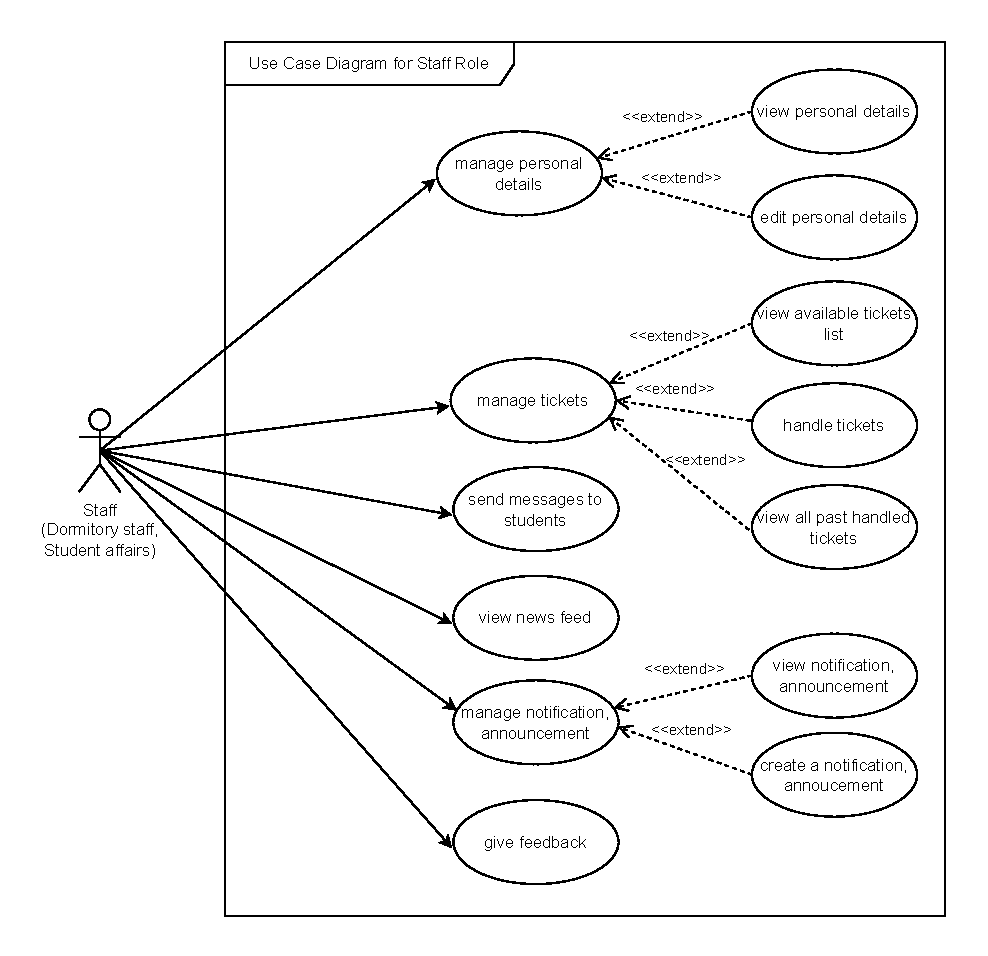
\includegraphics[width=0.9\columnwidth]{graphics/staff use case.pdf}
		\caption{Staff (Dormitory staff, Student affairs) Use Case Diagram}
		\label{fig:staff-use-case}
	\end{figure}
	
	
	
	\begin{figure}[H]
		\centering
		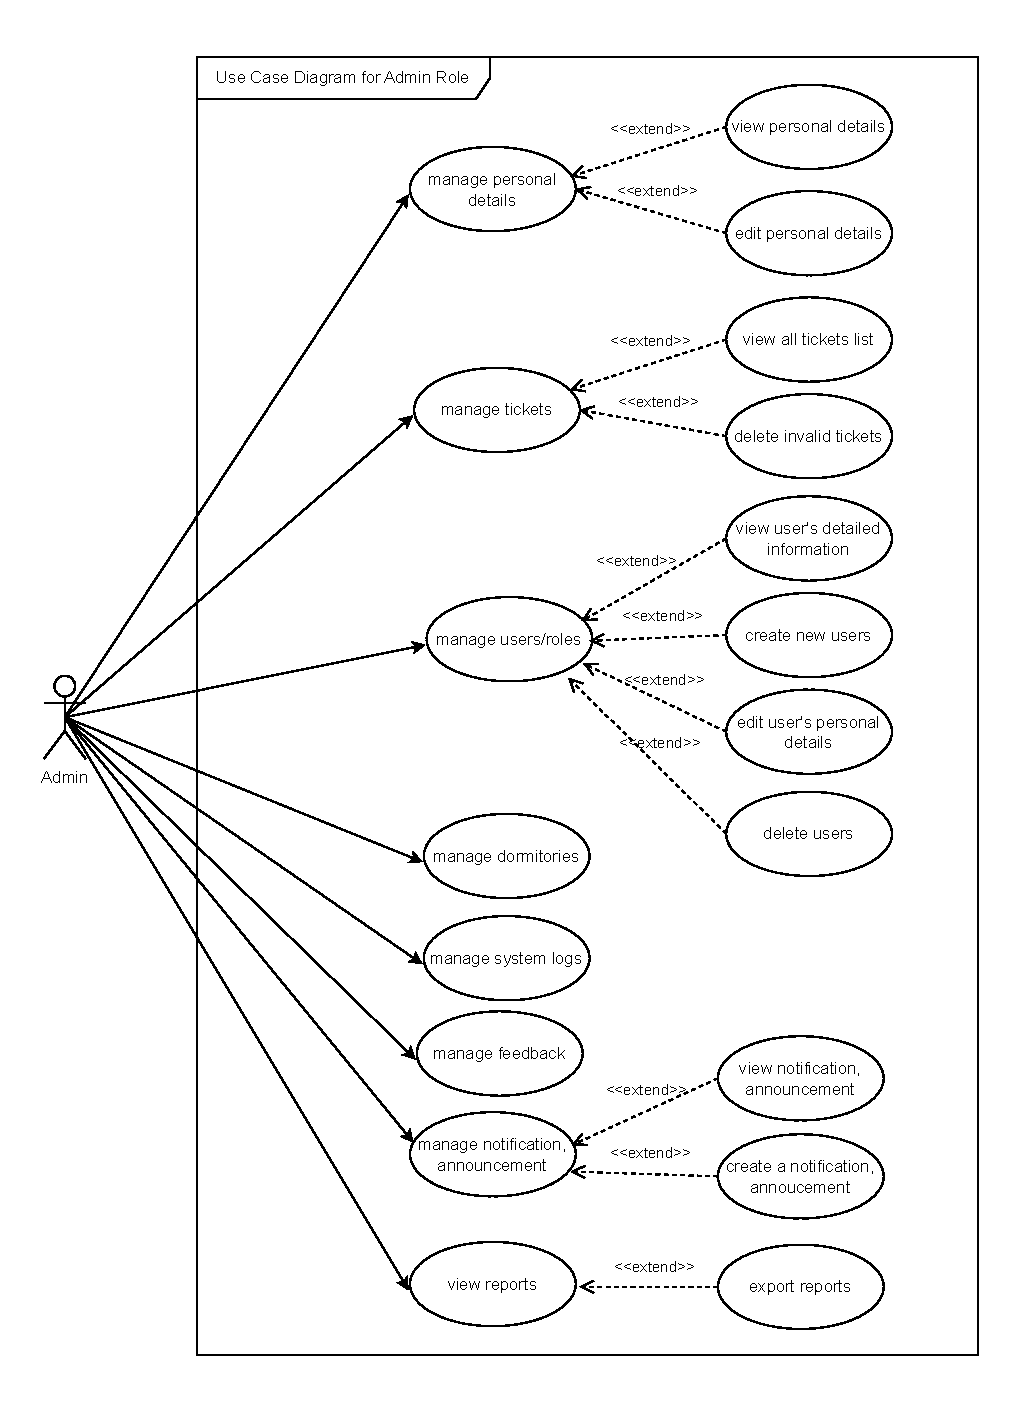
\includegraphics[width=0.84\columnwidth]{graphics/admin-use-case.pdf}
		\caption{Admin Use Case Diagram}
		\label{fig:admin-use-case}
	\end{figure}
	
	
\subsection{Process Workflow Diagrams}	
The core functionality of the Student Life Support Service is its ticket-raising process. The following diagram provides a detailed step-by-step illustration of this process.


\begin{figure}[H]
	\centering
	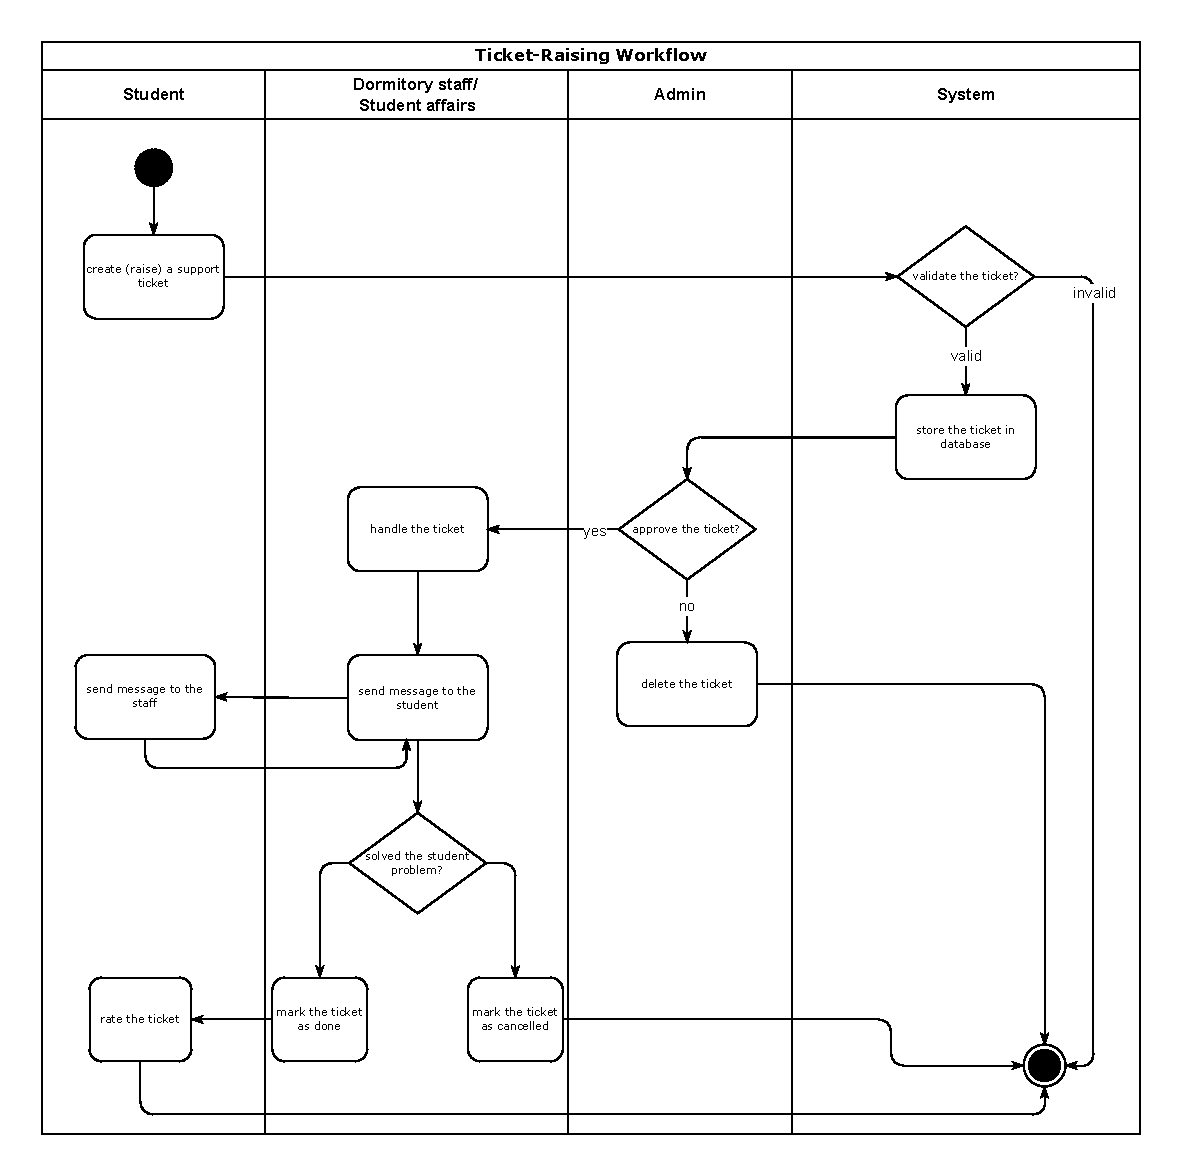
\includegraphics[width=1\columnwidth]{graphics/sys-workflow.pdf}
	\caption{Ticket-Raising Process Workflow}
	\label{fig:ticket-raising-workflow}
\end{figure}


\subsection{Database Design}
	\subsubsection{ER Diagram}
	\begin{figure}[H]
		\centering
		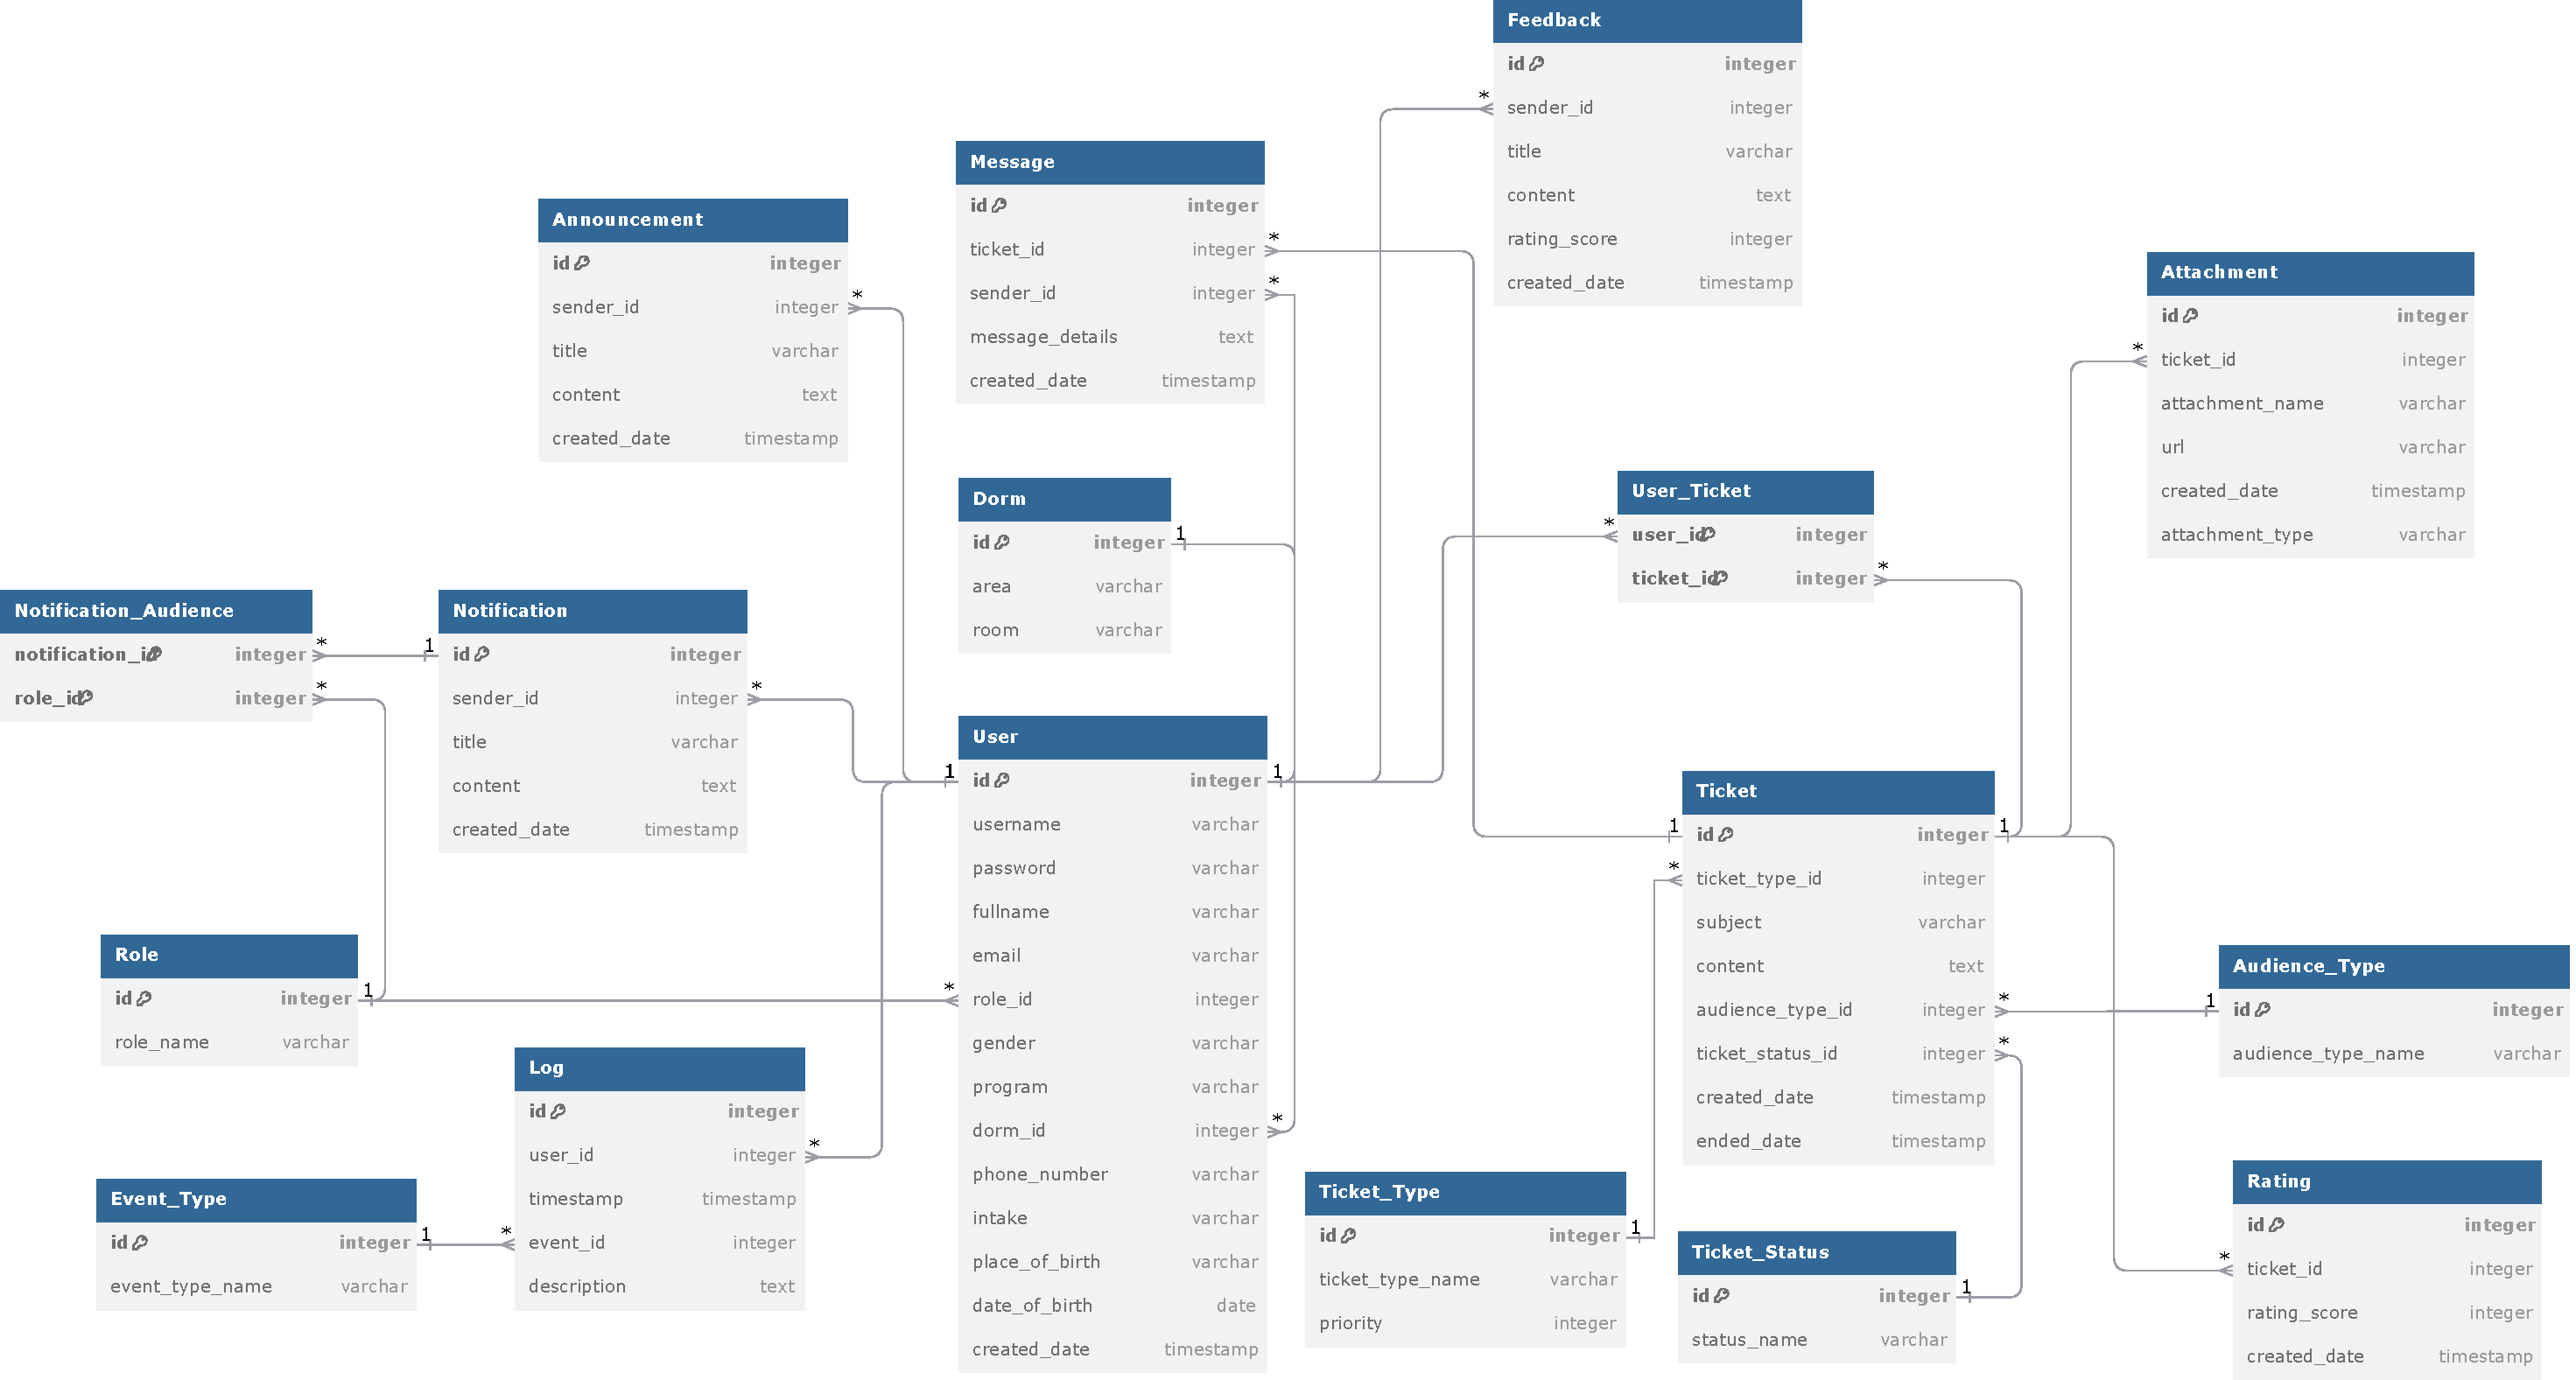
\includegraphics[width=1 \columnwidth]{graphics/er-diagram-v2.pdf}
		\caption{ER Diagram}
		\label{fig:er-diagram}
	\end{figure}


	\subsubsection{User Entity}
%	\newcolumntype{L}{>{\arraybackslash}m{3.5cm}}
	The User entity is fundamental to the system's user management, encompassing essential information that defines each user’s profile and access rights. This entity includes several key attributes that contribute to its operational integrity (see Table \ref{tab:user-entity})
	
	
	
	\begin{longtable}{|m{1.4cm}|m{2.8cm}|m{2.3cm}|m{2.3cm}|m{7.2cm}|}
		\hline
		\textbf{Key Type} & \textbf{Field Name} & \textbf{Data Type}                                                                                                                            & \textbf{Constraints} & \textbf{Description}   \\ \hline
		\endhead
		
		Primary & id & serial (int) & \makecell[l]{NOT NULL} & id of a user \\ \hline
		 & username & varchar(255) & \makecell[l]{NOT NULL \\ UNIQUE} & the user name of a user, it could be matriculation number of a student \\ \hline
		 & email & varchar(255) & \makecell[l]{NOT NULL \\ UNIQUE} & the email of a user \\ \hline
		 & fullname & varchar(255) & \makecell[l]{NOT NULL} & the full name of a user \\ \hline
		 & gender & varchar(255) & \makecell[l]{NOT NULL} & the gender of a user \\ \hline
		 Foreign & role\_id & int & \makecell[l]{NOT NULL} & the role id of a user \\ \hline
		 Foreign & dorm\_id & int & \makecell[l]{NOT NULL} & the dorm id where user lives (if the user does not live in a dormitory, dorm\_id value equals to 1)\\ \hline
		 & program & varchar(255) &  & the program that user registered at university (E.g: Computer Science, Architecture, etc.)\\ \hline
		 & intake & varchar(255) &  & the time when a user registered a specific program at university (E.g: 2020, 2021, etc.)\\ \hline
		 & phone\_number & varchar(255) & \makecell[l]{NOT NULL} & the phone number of a user\\ \hline
		 & place\_of\_birth & varchar(255) & \makecell[l]{NOT NULL} & the birth place of a user\\ \hline
		 & date\_of\_birth & date & \makecell[l]{NOT NULL} & the birth date of a user\\ \hline
		 & password & varchar(255) & \makecell[l]{NOT NULL} & the password of a user (in hashed string) \\ \hline
		 & created\_date & \makecell[l]{timestamp \\with time \\zone} & NOT NULL & the date time when a user account is created in the system \\ \hline
		 
		
		\caption{User Entity}
		\label{tab:user-entity}
		
	\end{longtable}
	
	
	
	
	\subsubsection{Ticket Entity}
	This table outlines the key attributes necessary for managing ticket entities within the system. It includes various fields such as the ticket ID, type, subject, content, and associated status. Additionally, it specifies data types, constraints, and a detailed description of each field to ensure proper handling of ticket information (refer to Table \ref{tab:ticket-entity}).
	
	
	
	\begin{longtable}{|m{1.4cm}|m{3.3cm}|m{2.3cm}|m{2.3cm}|m{6.7cm}|}
		\hline
		\textbf{Key Type} & \textbf{Field Name} & \textbf{Data Type}                                                                                                                            & \textbf{Constraints} & \textbf{Description}   \\ \hline
		\endhead
		
		Primary & id & serial (int) & \makecell[l]{NOT NULL} & id of a ticket \\ \hline
		Foreign & ticket\_type\_id & int & \makecell[l]{NOT NULL} & the id of the ticket type \\ \hline
		 & subject & varchar(255) & \makecell[l]{NOT NULL} & the subject (title) the ticket \\ \hline
		 & content & text & \makecell[l]{NOT NULL} & the detailed description of the problem declared in the ticket \\ \hline
		Foreign & audience\_type\_id & int & \makecell[l]{NOT NULL} & the id of audience type assigned to the ticket \\ \hline
		Foreign & ticket\_status\_id & int & \makecell[l]{NOT NULL} & the id of current status assigned to the ticket \\ \hline
		& created\_date & \makecell[l]{timestamp \\with time \\zone} & NOT NULL & the date time when a ticket is created in the system \\ \hline
		& ended\_date & \makecell[l]{timestamp \\with time \\zone} & NOT NULL & the date time when a ticket is marked as done or cancelled in the system \\ \hline
		
		
		\caption{Ticket Entity}
		\label{tab:ticket-entity}
		
	\end{longtable}
	
	
	\subsubsection{User\_Ticket Relationship}
	
		\begin{longtable}{|m{1.4cm}|m{3.3cm}|m{2.3cm}|m{2.3cm}|m{6.7cm}|}
			\hline
			\textbf{Key Type} & \textbf{Field Name} & \textbf{Data Type}                                                                                                                            & \textbf{Constraints} & \textbf{Description}   \\ \hline
			\endhead
			
			Primary & user\_id & int & \makecell[l]{NOT NULL} & id of a ticket \\ \hline
			
			Primary & ticket\_id & int & \makecell[l]{NOT NULL} & id of a user \\ \hline

			\caption{User\_Ticket Relationship}
			\label{tab:user-ticket}
			
		\end{longtable}
		
		This table describes the relationship between users and tickets within the system. It contains two primary key fields: \texttt{user\_id} and \texttt{ticket\_id}, each identified by a unique integer. The \texttt{user\_id} represents the unique identifier for a user, while the \texttt{ticket\_id} corresponds to a unique ticket within the system. Both fields are non-nullable, ensuring that each user and ticket association is properly recorded and maintained (refer to Table \ref{tab:user-ticket}). This relationship is essential for tracking which users have raised and handled specific tickets in the system .
	
	
	\subsubsection{Ticket\_Type Entity}
	The Ticket\_Type entity serves to classify different categories of tickets within the system, each defined by a unique identifier and a descriptive name. It also includes a priority level that indicates the urgency of each ticket type, where a higher value corresponds to a lower priority. This structure enables efficient ticket management and prioritization (see Table \ref{tab:ticket-type}).
	
	\begin{longtable}{|m{1.4cm}|m{3.3cm}|m{2.3cm}|m{2.3cm}|m{6.7cm}|}
		\hline
		\textbf{Key Type} & \textbf{Field Name} & \textbf{Data Type}                                                                                                                            & \textbf{Constraints} & \textbf{Description}   \\ \hline
		\endhead
		
		Primary & id & serial (int) & \makecell[l]{NOT NULL} & id of a ticket type \\ \hline
		 & ticket\_type\_name & varchar(255) & \makecell[l]{NOT NULL \\ UNIQUE} & the type name of a ticket \\ \hline
		
		& priority & int & \makecell[l]{NOT NULL} & the priority of the ticket type (higher indicates lower priority) \\ \hline
		
		\caption{Ticket\_Type Entity}
		\label{tab:ticket-type}
		
	\end{longtable}
	
%	This table defines the Ticket\_Type entity, which represents various types of tickets that can be created within the system. It consists of three fields:
%
%	\begin{itemize}
%		\item The \texttt{id} field, which is a primary key, represented as a serial integer, serving as the unique identifier for each ticket type.
%		
%		\item The \texttt{ticket\_type\_name} field, stored as a \texttt{varchar(255)}, holds the name of the ticket type, such as "Lost items" or "Harassment".
%		
%		\item The \texttt{priority} field, an integer, determines the urgency level of the ticket type, where a higher number indicates lower priority.
%	\end{itemize}
%	
%	\noindent All fields are marked as \texttt{NOT NULL}, ensuring that every ticket type has a unique identifier, name, and priority level. This structure is essential for organizing and managing different categories of support tickets in the system (refer to Table \ref{tab:ticket-type}).
	
	
	
	\subsubsection{Ticket\_Status Entity}
	The Ticket\_Status entity is designed to define various states that a ticket can be in within the system. Each status is uniquely identified by an ID and has a descriptive name, allowing for clear tracking and management of tickets throughout their lifecycle. This structured approach enhances the ability to monitor ticket progress and provides clarity to users regarding the current status of their tickets (see Table \ref{tab:ticket-status}).
	
	\begin{longtable}{|m{1.4cm}|m{3.3cm}|m{2.3cm}|m{2.3cm}|m{6.7cm}|}
		\hline
		\textbf{Key Type} & \textbf{Field Name} & \textbf{Data Type}                                                                                                                            & \textbf{Constraints} & \textbf{Description}   \\ \hline
		\endhead
		
		Primary & id & serial (int) & \makecell[l]{NOT NULL} & id of a ticket status \\ \hline
		& status\_name & varchar(255) & \makecell[l]{NOT NULL \\ UNIQUE} & the status name of a ticket \\ \hline
		
		\caption{Ticket\_Status Entity}
		\label{tab:ticket-status}
		
	\end{longtable}
	
	
%	This table describes the Ticket\_Status entity, which is used to represent the current status of a support ticket within the system. It contains two fields:
%	
%	
%	\begin{enumerate}
%		
%		\item The \texttt{id} field is the primary key, defined as a serial integer, serving as the unique identifier for each ticket status. This field is essential for distinguishing between different statuses.
%		
%		\item The \texttt{status\_name} field is a \texttt{varchar(255)} that stores the name of the ticket status, such as "pending," "in progress," "done," or "cancelled." These status names provide insight into the progress of each support ticket.
%	\end{enumerate}
%	
%	\noindent Both fields are marked as \texttt{NOT NULL}, ensuring that every ticket status has a unique identifier and name, which is crucial for tracking and managing the lifecycle of tickets (refer to Table \ref{tab:ticket-status}).
	
	
	
	\subsubsection{Audience\_Type Entity}
	
	The Audience\_Type entity categorizes target audiences for tickets in the system. Each type is uniquely identified by an ID and has a descriptive name, enhancing communication and ticket management for specific user groups (see Table \ref{tab:audience-type}).
	
	\begin{longtable}{|m{1.4cm}|m{3.8cm}|m{2.3cm}|m{2.3cm}|m{6.2cm}|}
		\hline
		\textbf{Key Type} & \textbf{Field Name} & \textbf{Data Type}                                                                                                                            & \textbf{Constraints} & \textbf{Description}   \\ \hline
		\endhead
		
		Primary & id & serial (int) & \makecell[l]{NOT NULL} & id of a ticket audience type \\ \hline
		& audience\_type\_name & varchar(255) & \makecell[l]{NOT NULL \\ UNIQUE} & the target audience type name of a ticket \\ \hline
		
		\caption{Audience\_Type Entity}
		\label{tab:audience-type}
		
	\end{longtable}
	
	
%	This table outlines the Audience\_Type entity, which is used to categorize the audience for support tickets within the system. It includes two fields:
%	
%	\begin{itemize}
%		\item The \texttt{id} field, which is the primary key, is a serial integer that uniquely identifies each audience type. This field ensures each audience type is distinct and traceable.
%		
%		\item The \texttt{audience\_type\_name} field is a \texttt{varchar(255)} that stores the name of the audience type for a ticket. It could be either "private" or "public," where public tickets are visible to other students, while private tickets are only visible to the ticket creator and assigned staff.
%	\end{itemize}
%	
%
%	\noindent Both fields are defined as NOT NULL, ensuring that each audience type has a unique identifier and a clearly defined type name, which is essential for managing ticket visibility (refer to Table \ref{tab:audience-type}).
%	
	
	
	\subsubsection{Attachment Entity}
	The Attachment entity manages files associated with tickets in the system. Each attachment is uniquely identified by an ID and linked to a specific ticket through a foreign key. The entity includes attributes for the original file name, its server \acs{url}, and the timestamp of its upload, ensuring organized storage and retrieval of related documents for user reference (see Table \ref{tab:attachment}).
	
	\begin{longtable}{|m{1.4cm}|m{3.3cm}|m{2.3cm}|m{2.3cm}|m{6.3cm}|}
		\hline
		\textbf{Key Type} & \textbf{Field Name} & \textbf{Data Type}                                                                                                                            & \textbf{Constraints} & \textbf{Description}   \\ \hline
		\endhead
		
		Primary & id & serial (int) & \makecell[l]{NOT NULL} & id of an attachment \\ \hline
		Foreign & ticket\_id & int & \makecell[l]{NOT NULL} & the reference ticket id which has an attachment \\ \hline
		 & attachment\_name & varchar(255) & \makecell[l]{NOT NULL} & the original name of the attachment \\ \hline
		 & url & varchar(255) & \makecell[l]{NOT NULL \\ UNIQUE} & the address of an attachment on the server  \\ \hline
		 & created\_date & \makecell[l]{timestamp \\with time \\zone} & NOT NULL & the date time when an attachment is firstly uploaded to the system \\ \hline
		
		\caption{Attachment Entity}
		\label{tab:attachment}
		
	\end{longtable}
	
%	The Attachment entity captures essential details about files associated with support tickets in the system. The table comprises the following key fields:
%	
%	\begin{itemize}
%		\item \texttt{id}: This primary key is a serial integer that uniquely identifies each attachment in the system, ensuring every file is traceable.
%		
%		\item \texttt{ticket\_id}: A foreign key linking the attachment to the specific ticket it belongs to, creating a clear relationship between files and their corresponding support tickets.
%		
%		\item \texttt{attachment\_name}: This field stores the original name of the file, providing users and administrators with a clear reference to the document.
%		
%		\item \texttt{url}: A \texttt{varchar(255)} field that holds the unique server address where the attachment is stored. It is constrained to be both \texttt{NOT NULL} and \texttt{UNIQUE}, ensuring each file is stored at a distinct location.
%		
%		\item \texttt{created\_date}: A timestamp with time zone that records the exact moment the attachment was uploaded to the system, offering important chronological information for ticket management.
%	\end{itemize}
%
%	\noindent This entity provides a robust structure for managing files, enabling easy access and secure storage of attachments related to user support requests (refer to Table \ref{tab:attachment}).
	
	
	
	\subsubsection{Rating Entity}
	The Rating entity captures user ratings for tickets in the system. Each rating is uniquely identified by an ID and linked to a specific ticket through a foreign key. It includes a score reflecting the user's assessment and a timestamp indicating when the rating was given, enabling effective tracking of user feedback (see Table \ref{tab:rating}).
	
	\begin{longtable}{|m{1.4cm}|m{2.5cm}|m{2.3cm}|m{2.3cm}|m{6.7cm}|}
		\hline
		\textbf{Key Type} & \textbf{Field Name} & \textbf{Data Type}                                                                                                                            & \textbf{Constraints} & \textbf{Description}   \\ \hline
		\endhead
		
		Primary & id & serial (int) & \makecell[l]{NOT NULL} & id of a rating \\ \hline
		Foreign & ticket\_id & int & \makecell[l]{NOT NULL} & the reference ticket id which has the rating \\ \hline
		& rating\_score & int & \makecell[l]{NOT NULL} & the rating score of a ticket \\ \hline
		& created\_date & \makecell[l]{timestamp \\with time \\zone} & NOT NULL & the date time when user rates a ticket. \\ \hline
		
		\caption{Rating Entity}
		\label{tab:rating}
		
	\end{longtable}
	
%	The Rating entity is designed to capture and store feedback from users regarding their support tickets. This table includes several key fields:
%	
%	\begin{itemize}
%		\item \texttt{id}: A serial integer serving as the primary key, which uniquely identifies each rating entry in the system.
%		
%		\item \texttt{ticket\_id}: A foreign key that links the rating to the specific ticket being evaluated, ensuring that every rating is associated with a particular support request.
%		
%		\item \texttt{rating\_score}: A number field that holds the actual score or feedback provided by the user. This score reflects the user's level of satisfaction with the handling of their ticket.
%		
%		\item \texttt{created\_date}: A timestamp with time zone indicating when the rating was submitted, allowing for tracking and auditing of feedback over time.
%	\end{itemize}
%	
%	\noindent This entity is crucial for maintaining a structured and traceable system for user feedback, enabling continuous service improvement based on user satisfaction (refer to Table \ref{tab:rating}).
	
	
	
	\subsubsection{Feedback Entity}
	
	The Feedback entity collects user feedback on various aspects of the system. Each feedback entry is uniquely identified by an ID and linked to the user providing it through a foreign key. It includes a title for the feedback, detailed content, a rating score reflecting the user's evaluation, and a timestamp indicating when the feedback was submitted. This structure facilitates the collection and analysis of user opinions to enhance system performance (see Table \ref{tab:feedback}).
	
	\begin{longtable}{|m{1.4cm}|m{2.5cm}|m{2.3cm}|m{2.3cm}|m{6.7cm}|}
		\hline
		\textbf{Key Type} & \textbf{Field Name} & \textbf{Data Type}                                                                                                                            & \textbf{Constraints} & \textbf{Description}   \\ \hline
		\endhead
		
		Primary & id & serial (int) & \makecell[l]{NOT NULL} & id of a feedback \\ \hline
		Foreign & sender\_id & int & \makecell[l]{NOT NULL} & the id of the user who gives the feedback \\ \hline
		& title & varchar(255) & \makecell[l]{NOT NULL} & the title (subject) of the feedback \\ \hline
		& content & text & \makecell[l]{NOT NULL} & the details of the feedback \\ \hline
		& rating\_score & int & \makecell[l]{NOT NULL} & the rating score of the feedback \\ \hline
		& created\_date & \makecell[l]{timestamp \\with time \\zone} & NOT NULL & the date time when user gives the feedback. \\ \hline
		
		\caption{Feedback Entity}
		\label{tab:feedback}
		
	\end{longtable}
%	
%	The Feedback entity is structured to store user feedback, enabling users to provide detailed evaluations of the system. It consists of several key fields:
%	
%	\begin{itemize}
%		\item \texttt{id}: A serial integer that serves as the primary key, uniquely identifying each feedback entry.
%		
%		\item \texttt{sender\_id}: A foreign key representing the user who submits the feedback, ensuring proper linkage between the feedback and its author.
%		
%		\item \texttt{title}: A \texttt{varchar(255)} field that contains the subject or title of the feedback, summarizing the main point of the user's input.
%		
%		\item \texttt{content}: A text field used for the detailed explanation of the feedback, where users can elaborate on their experience or suggestions.
%		
%		\item \texttt{rating\_score}: An integer representing the overall rating score associated with the feedback, allowing users to quantify their level of satisfaction.
%		
%		\item \texttt{created\_date}: A timestamp with time zone capturing when the feedback was submitted, which aids in tracking and analysis over time.
%	\end{itemize}
%	
%	\noindent This entity is critical for gathering and storing user insights, helping administrators to improve the system based on user evaluations and suggestions (refer to Table \ref{tab:feedback}).
	
	
	
	\subsubsection{Message Entity}
	The Message entity stores individual messages associated with tickets within the system. Each message is identified by a unique ID and linked to a specific ticket through a foreign key, effectively acting as a conversation identifier. It records the sender's ID, the content of the message, and a timestamp indicating when the message was sent. This structure supports organized communication related to tickets, enabling users to track conversations effectively (see Table \ref{tab:message}).
	
	\begin{longtable}{|m{1.4cm}|m{2.9cm}|m{2.3cm}|m{2.3cm}|m{6.7cm}|}
		\hline
		\textbf{Key Type} & \textbf{Field Name} & \textbf{Data Type}                                                                                                                            & \textbf{Constraints} & \textbf{Description}   \\ \hline
		\endhead
		
		Primary & id & serial (int) & \makecell[l]{NOT NULL} & id of a message \\ \hline
		Foreign & ticket\_id & int & \makecell[l]{NOT NULL} & the id of a ticket which has the message (acts as a conversation id) \\ \hline
		& sender\_id & int & \makecell[l]{NOT NULL} & id of a user who has the message \\ \hline
		& message\_details & text & \makecell[l]{NOT NULL} & the details of a message \\ \hline
		& created\_date & \makecell[l]{timestamp \\with time \\zone} & NOT NULL & the date time when user send a message. \\ \hline
		
		\caption{Message Entity}
		\label{tab:message}
		
	\end{longtable}
	
	
	
%	The Message entity is designed to store and manage the communication between users related to a specific ticket, acting as the foundation for the system's real-time messaging feature. The key components of this entity include:
%	
%	\begin{itemize}
%		\item \texttt{id}: A serial integer that uniquely identifies each message, serving as the primary key.
%		
%		\item \texttt{ticket\_id}: A foreign key that links the message to a specific ticket, representing the conversation associated with that ticket.
%		
%		\item \texttt{sender\_id}: This field stores the id of the user who sent the message, ensuring proper identification of the sender.
%		
%		\item \texttt{message\_details}: A text field that contains the content of the message, capturing the full details of the communication.
%		
%		\item \texttt{created\_date}: A timestamp with time zone that records when the message was sent, which helps in tracking the conversation timeline.
%	\end{itemize}
%	
%	\noindent This entity is essential for facilitating and managing user interactions within the system's ticketing process, ensuring seamless communication between users (refer to Table \ref{tab:message}).
	
	
	
	\subsubsection{Dorm Entity}
	The Dorm entity represents the various dormitories within the system. Each dormitory is uniquely identified by an ID and includes details about its area and specific room designation. This structure facilitates the organization and management of dormitory accommodations, ensuring that each location is easily identifiable (see Table \ref{tab:dorm}).
	
	
	\begin{longtable}{|m{1.4cm}|m{2.5cm}|m{2.3cm}|m{2.3cm}|m{6.7cm}|}
		\hline
		\textbf{Key Type} & \textbf{Field Name} & \textbf{Data Type}                                                                                                                            & \textbf{Constraints} & \textbf{Description}   \\ \hline
		\endhead
		
		Primary & id & serial (int) & \makecell[l]{NOT NULL} & id of a dorm \\ \hline
		& area & varchar(255) & \makecell[l]{NOT NULL \\ UNIQUE} & the dorm area name  \\ \hline
		& room & varchar(255) & \makecell[l]{NOT NULL \\ UNIQUE} & the dorm room of an area \\ \hline
		
		\caption{Dorm Entity}
		\label{tab:dorm}
		
	\end{longtable}
	
%	The Dorm entity is a crucial component of the system, designed to encapsulate and manage information related to student accommodation within the dormitory facilities. This entity comprises the following key attributes:
%	
%	
%	\begin{itemize}
%		\item \texttt{id}: This field serves as the primary key and is defined as a serial integer, uniquely identifying each dorm entry in the database.
%		
%		\item \texttt{area}: A varchar field that stores the name of the dorm area. This field is marked as NOT NULL and UNIQUE, ensuring that each area name is distinct and cannot be left empty, thereby preventing duplicate entries.
%		
%		\item \texttt{room}: Similar to the area field, this varchar field holds the specific room identifier within the dormitory. It is also marked as NOT NULL and UNIQUE, ensuring that each room name is unique and that no room entries can be left undefined.
%	\end{itemize}
%
%	
%	\noindent This structured representation of dormitory information is vital for effective accommodation management, allowing for easy tracking and organization of dorm areas and their respective rooms (see Table \ref{tab:dorm}).
	
	
	
	
	\subsubsection{Announcement Entity}
	The Announcement entity captures information about announcements made within the system. Each announcement is uniquely identified by an ID and includes details such as the sender's ID, title, content, and the timestamp of when it was created. This structure enables effective communication and dissemination of important information among users (see Table \ref{tab:announcement}).
	
	\begin{longtable}{|m{1.4cm}|m{2.5cm}|m{2.3cm}|m{2.3cm}|m{6.7cm}|}
		\hline
		\textbf{Key Type} & \textbf{Field Name} & \textbf{Data Type}                                                                                                                            & \textbf{Constraints} & \textbf{Description}   \\ \hline
		\endhead
		
		Primary & id & serial (int) & \makecell[l]{NOT NULL} & id of an announcement \\ \hline
		Foreign & sender\_id & int & \makecell[l]{NOT NULL} & the id of user who sends the announcement  \\ \hline
		& title & varchar(255) & \makecell[l]{NOT NULL} & the title of an announcement \\ \hline
		& content & text & \makecell[l]{NOT NULL} & the details of an announcement \\ \hline
		& created\_date & \makecell[l]{timestamp \\with time \\zone} & NOT NULL & the date time when user sends an announcement. \\ \hline
		
		\caption{Announcement Entity}
		\label{tab:announcement}
		
	\end{longtable}
	
	
%	The Announcement entity is integral to the communication framework of the system, facilitating the dissemination of important information to users. This entity encompasses several key attributes that define its structure and functionality:
%	
%	\begin{itemize}
%		\item \texttt{id}: This field acts as the primary key for the announcement entity and is defined as a serial integer. It uniquely identifies each announcement within the database, ensuring that each entry is distinct.
%		
%		\item \texttt{sender\_id}: This foreign key field references the user who initiates the announcement. It is an integer marked as \texttt{NOT NULL}, ensuring that every announcement is attributed to a specific user.
%		
%		\item \texttt{title}: A \texttt{varchar} field that holds the title of the announcement. This field is also marked as NOT NULL, requiring a descriptive title for each announcement to enhance clarity and accessibility for users.
%		
%		\item \texttt{content}: This text field captures the detailed message of the announcement. It is crucial for providing comprehensive information and is marked as NOT NULL, ensuring that all announcements contain substantive content.
%		
%		\item \texttt{created\_date}: Defined as a timestamp with time zone, this field records the exact date and time when the announcement is sent. Marked as NOT NULL, it ensures that every announcement is time-stamped for reference.
%	\end{itemize}
%
%	
%	\noindent The structured nature of the Announcement entity enhances the system's ability to communicate effectively with its users, allowing for clear and organized dissemination of important information (see Table \ref{tab:announcement}).
	
	
	\subsubsection{Notification Entity}
	The Notification entity records details about notifications sent within the system. Each notification is uniquely identified by an ID and includes information such as the sender's ID, title, content, and the timestamp of when it was created. This structure supports timely communication and updates for users (see Table \ref{tab:notification}).
	
	\begin{longtable}{|m{1.4cm}|m{2.5cm}|m{2.3cm}|m{2.3cm}|m{6.7cm}|}
		\hline
		\textbf{Key Type} & \textbf{Field Name} & \textbf{Data Type}                                                                                                                            & \textbf{Constraints} & \textbf{Description}   \\ \hline
		\endhead
		
		Primary & id & serial (int) & \makecell[l]{NOT NULL} & id of a notification \\ \hline
		Foreign & sender\_id & int & \makecell[l]{NOT NULL} & the id of user who sends the notification  \\ \hline
		& title & varchar(255) & \makecell[l]{NOT NULL} & the title of a notification \\ \hline
		& content & text & \makecell[l]{NOT NULL} & the details of a notification \\ \hline
		& created\_date & \makecell[l]{timestamp \\with time \\zone} & NOT NULL & the date time when user sends a notification. \\ \hline
		
		\caption{Notification Entity}
		\label{tab:notification}
		
	\end{longtable}
	
	
%	The Notification entity plays a critical role in the system's communication mechanism, ensuring that important alerts and updates reach users in a timely manner. This entity is structured with several key attributes that facilitate its functionality and organization:
%	
%	\begin{itemize}
%		\item \texttt{id}: This primary key, defined as a serial integer, uniquely identifies each notification within the database, ensuring that all records are distinct and easily retrievable.
%		
%		\item \texttt{sender\_id}: A foreign key field that references the user who initiates the notification. It is marked as \texttt{NOT NULL}, ensuring that every notification is associated with a specific user, which aids in accountability and context.
%		
%		\item \texttt{title}: This \texttt{varchar} field holds the title of the notification. It is also marked as \texttt{NOT NULL}, requiring each notification to have a descriptive title, thus enhancing clarity and user engagement.
%		
%		\item \texttt{content}: A text field that captures the detailed message of the notification. Marked as \texttt{NOT NULL}, this attribute ensures that all notifications provide comprehensive information for users.
%		
%		\item \texttt{created\_date}: Defined as a timestamp with time zone, this field records the exact date and time when the notification is sent. Marked as \texttt{NOT NULL}, it ensures that each notification is time-stamped, allowing for accurate tracking and historical reference.
%	\end{itemize}
%	
%	\noindent The structured attributes of the Notification entity bolster the system's capability to deliver timely and relevant updates, facilitating effective communication among users (see Table \ref{tab:notification}).
	
	
	
	\subsubsection{Role Entity}
	The Role entity is crucial for defining user permissions and access levels within the system. This entity facilitates the management of user roles, ensuring that access rights are clearly delineated and easily maintained (see Table \ref{tab:role}).
	
	\begin{longtable}{|m{1.4cm}|m{2.5cm}|m{2.3cm}|m{2.3cm}|m{6.7cm}|}
		\hline
		\textbf{Key Type} & \textbf{Field Name} & \textbf{Data Type}                                                                                                                            & \textbf{Constraints} & \textbf{Description}   \\ \hline
		\endhead
		
		Primary & id & serial (int) & \makecell[l]{NOT NULL} & id of a role \\ \hline
		 & role\_name & varchar(255) & \makecell[l]{NOT NULL} & the name of a role  \\ \hline
		
		\caption{Role Entity}
		\label{tab:role}
		
	\end{longtable}
	
	
	
	
	\subsubsection{Notification\_Audience Relationship}
	
	The Notification\_Audience relationship establishes a many-to-many association between notifications and user roles, defining which roles are eligible to receive specific notifications. This structure enhances targeted communication within the system, allowing for tailored information delivery based on user roles (see Table \ref{tab:notification-audience}).
	
	\begin{longtable}{|m{1.4cm}|m{2.7cm}|m{2.3cm}|m{2.3cm}|m{6.5cm}|}
		\hline
		\textbf{Key Type} & \textbf{Field Name} & \textbf{Data Type}                                                                                                                            & \textbf{Constraints} & \textbf{Description}   \\ \hline
		\endhead
		
		Primary & notification\_id & int & \makecell[l]{NOT NULL} & id of a notification \\ \hline
		Primary & role\_id & int & \makecell[l]{NOT NULL} & the id of a role  \\ \hline
		
		\caption{Notification\_Audience Entity}
		\label{tab:notification-audience}
		
	\end{longtable}
	
	
	
	
	
	
	\subsubsection{Log Entity}
	
	The Log entity serves as a critical component for tracking user actions and system events within the application. It records essential information, including the user involved, the specific event associated with the action, a detailed description, and the timestamp of when the log entry was created. This structured approach enables effective auditing and monitoring of system activities (see Table \ref{tab:log}).
	
	
	\begin{longtable}{|m{1.4cm}|m{2.5cm}|m{2.3cm}|m{2.3cm}|m{6.7cm}|}
		\hline
		\textbf{Key Type} & \textbf{Field Name} & \textbf{Data Type}                                                                                                                            & \textbf{Constraints} & \textbf{Description}   \\ \hline
		\endhead
		
		Primary & id & serial (int) & \makecell[l]{NOT NULL} & id of a log \\ \hline
		Foreign & user\_id & int & \makecell[l]{NOT NULL} & the reference user who has actions on log  \\ \hline
		Foreign & event\_id & int & \makecell[l]{NOT NULL} & the id of an event  \\ \hline
		 & description & text & \makecell[l]{NOT NULL} & the details of a log  \\ \hline
		 & timestamp & \makecell[l]{timestamp \\with time \\zone} & NOT NULL & the date time when a log is written to the database. \\ \hline
		
		\caption{Log Entity}
		\label{tab:log}
		
	\end{longtable}
	
	
	
	
	\subsubsection{Event\_Type Entity}
	The Event\_Type entity is designed to categorize various system events, providing a structured framework for event classification. It includes unique identifiers for each event type, along with descriptive names that facilitate easy reference and management within the system. This organization enhances the overall functionality and tracking of system activities (see Table \ref{tab:event-type}).
	
	\begin{longtable}{|m{1.4cm}|m{3.3cm}|m{2.3cm}|m{2.3cm}|m{6cm}|}
		\hline
		\textbf{Key Type} & \textbf{Field Name} & \textbf{Data Type}                                                                                                                            & \textbf{Constraints} & \textbf{Description}   \\ \hline
		\endhead
		
		Primary & id & serial (int) & \makecell[l]{NOT NULL} & id of a system event type \\ \hline
		 & event\_type\_name & varchar(255) & \makecell[l]{NOT NULL \\ UNIQUE} & the name of a system event type  \\ \hline

		\caption{Event\_Type Entity}
		\label{tab:event-type}
		
	\end{longtable}
	
	

\subsection{System Architecture}

	\subsubsection{Overview}
	
	The system follows a three-tier architecture, consisting of the following layers:
	
	\begin{figure}[H]
		\centering
		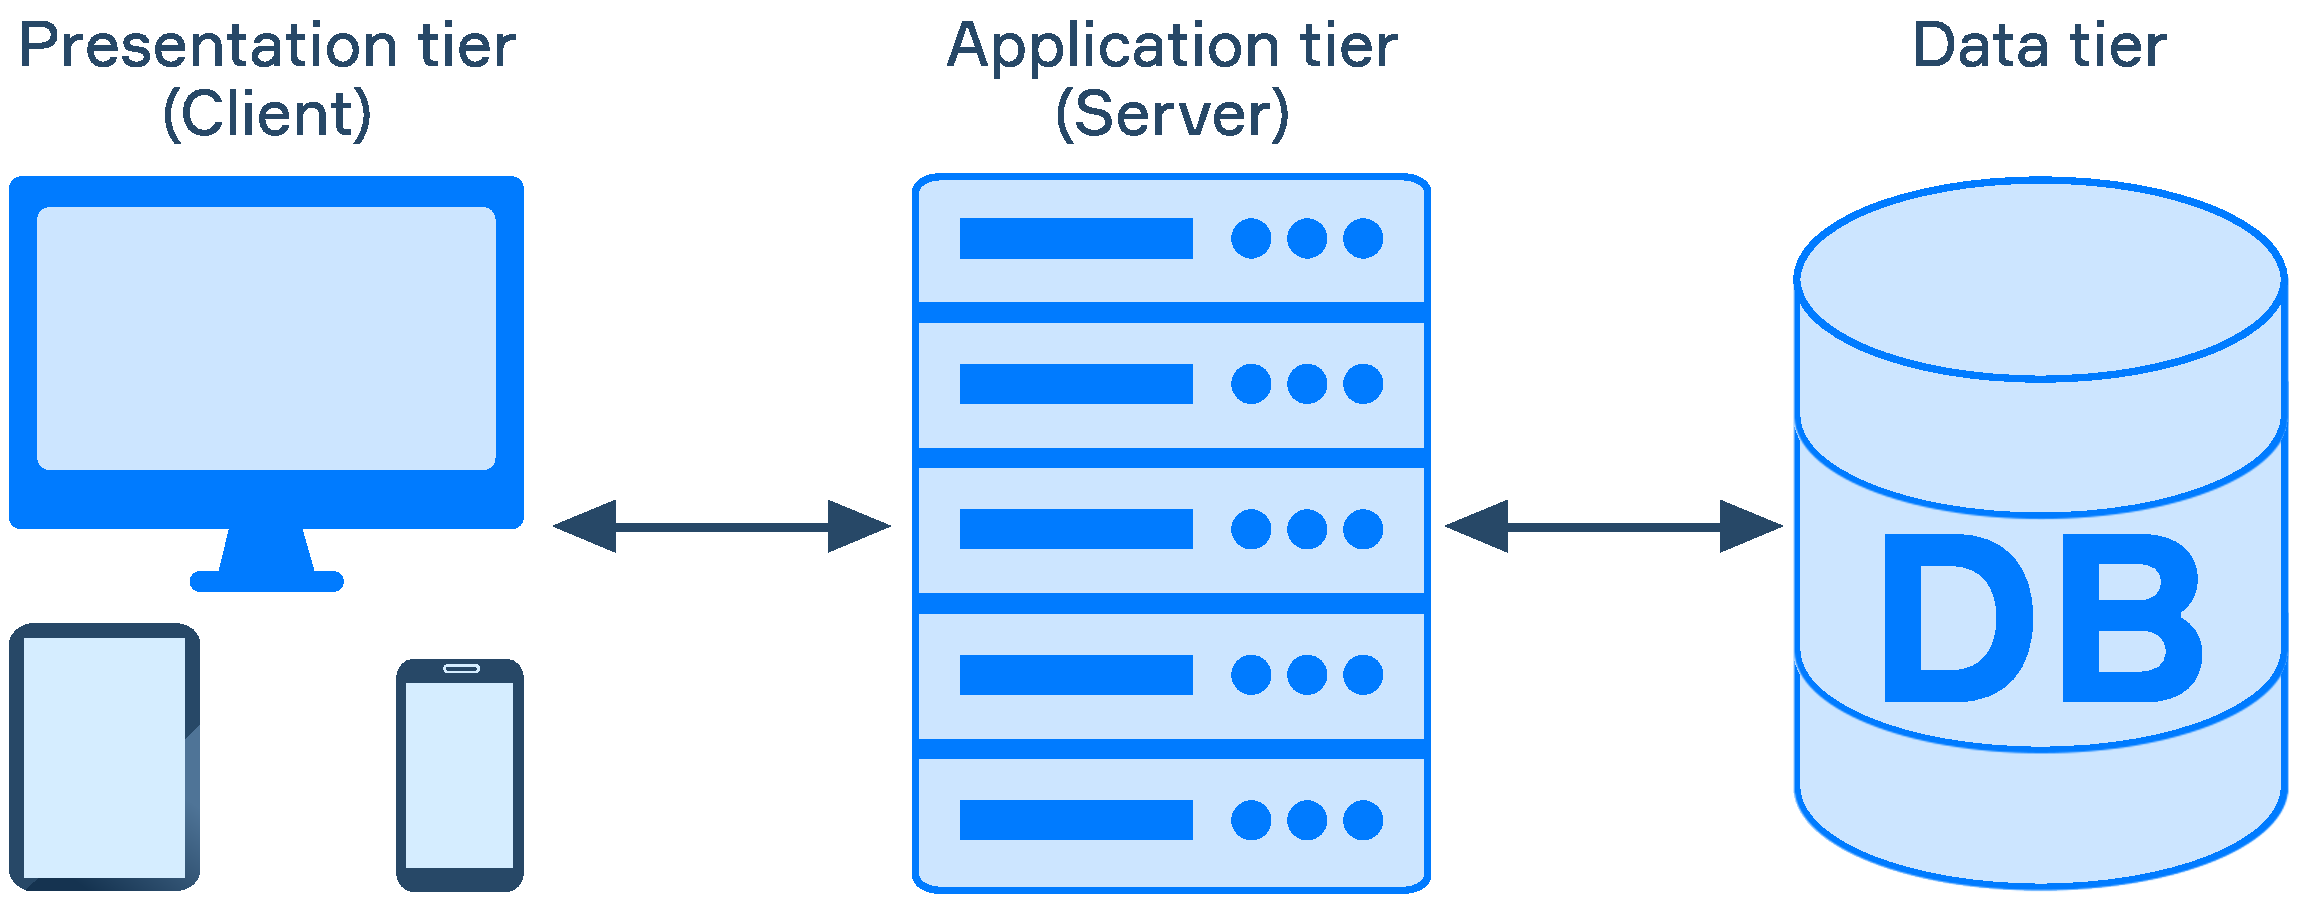
\includegraphics[width=0.7\columnwidth]{graphics/3-tier-arch.pdf}
		\caption{Three-tier Architecture \cite{3-tier}}
		\label{fig:3-tier}
	\end{figure}
	
	
	\begin{enumerate}
		\item \textbf{Presentation Layer (Client):}
		
		Handles all interactions with the user.
		Implements the user interface using ReactJS and Material UI.
		Communicates with the server through RESTful API calls and SocketIO for real-time features.
		Responsible for rendering components, collecting user input, and displaying data received from the backend.
		
		\item \textbf{Business Logic Layer (Server)}:
		
		NodeJS and ExpressJS handle the core business logic, such as processing support ticket requests, authenticating users, managing roles, and communicating with the database.
		SocketIO is used to manage real-time messaging between students and staff.
		Implements security features like JWT-based authentication and session management using Redis.
		
		\item \textbf{ Data Layer (Database)}:
		
		PostgreSQL stores all persistent data, including user profiles, support tickets, messages, and system logs.
		The server communicates with the database using SQL queries to retrieve, create, update, and delete records.
		Ensures data consistency and integrity by enforcing constraints, foreign keys, and relationships.
		
	\end{enumerate}
	
	
	\subsubsection{3-Tier Architecture Implementation}
	
	\begin{longtable}{|m{4cm}|m{13cm}|}
		\hline
		
		
		Presentation Layer & The frontend is built using ReactJS, Material UI, and Vite. These technologies allow for dynamic rendering, responsive design, and a user-friendly interface. The presentation layer is responsible for capturing user input, displaying data, and providing real-time updates through WebSockets (using Socket.IO).  \\ \hline
		
		Business Logic Layer & The backend is implemented using NodeJS and ExpressJS. This layer handles all business logic, processes user requests, applies business rules, and interacts with the data layer. The business logic layer leverages Socket.IO for real-time communication, allowing instant messaging between students and staff.  \\ \hline
		
		Data Access Layer & The data access layer utilizes PostgreSQL to store user data, support ticket information, and system logs. The data layer interacts with the business logic layer to retrieve and store information as needed. Redis is employed for session management by storing the user JWT refresh token. \\ \hline

		
		\caption{3-Tier Architecture Implementation}
		\label{tab:3-tier-implement}
		
	\end{longtable}


\subsection{API Design}
The API (Application Programming Interface) design is crucial for enabling communication between the frontend and backend of the Student Life Support Service application. A well-structured API facilitates seamless data exchange and supports the application's functionalities. \\

	API Design Principles:
	\begin{itemize}
		\item \textbf{RESTful Architecture}: The API follows RESTful principles, utilizing standard HTTP methods (GET, POST, PATCH, DELETE) for interaction. This allows for clear and intuitive endpoints.
		
		\item \textbf{Versioning}: The API is versioned (/api/v1/) to manage changes and ensure backward compatibility for existing clients.
		
		\item \textbf{Error Handling}: Consistent error responses are defined, returning meaningful HTTP status codes (200 for success, 404 for not found, 500 for server errors) along with descriptive messages.
	\end{itemize}
	
	Data format:
	\begin{itemize}
		\item \textbf{Request Format}: All requests to the API are in JSON format, with the appropriate headers set (Content-Type: application/json).
		
		\item \textbf{Response Format}: API responses are standardized to return JSON objects. Successful responses include a status field, data field (for returned data), and an optional message field for additional context.
	\end{itemize}
	
	Security Measures: 
	\begin{itemize}
		\item JWT is used for user authentication, with tokens sent in the Authorization header of each request (Authorization: Bearer <token>).
	\end{itemize}

	\newpage 
	\subsubsection{Authentication/Authorization API}
	\begin{longtable}{|m{1.5cm}|m{4.8cm}|m{3.3cm}|m{3cm}|m{3.2cm}|}
		\hline
		\textbf{Method} & \textbf{Endpoint} & \textbf{Header}                                                                                                                            & \textbf{Request Body} & \textbf{Response / Description}   \\ \hline
		\endhead
		
		POST & /auth/login & Content-Type: application/json & JSON object with username and password & JSON object which contains access token, refresh token and general user information \\ \hline
		
		POST & /auth/logout & Authorization: Bearer <token>\newline Cookie: <refreshToken> & None  & Clear tokens and cookie \\ \hline
		
		POST & /auth/refresh-token & Cookie: <refreshToken>& None & JSON object which contains new access token \\ \hline
		
		POST & /auth/verify-refreshToken & Cookie: <refreshToken>& None & JSON object which contains validation status and message \\ \hline
		
		POST & /auth/reset-password &  Content-Type: application/json &  JSON object with email  &  JSON object which contains message \\ \hline
		
		PATCH & /auth/reset-password &  Content-Type: application/json &  JSON object with reset password token &  JSON object which contains message \\ \hline
		
		
		\caption{Authentication/Authorization API}
		\label{tab:auth-api}
		
	\end{longtable}
	
	
The Login API enables the client to authenticate with the server and obtain permissions based on the client’s role. Upon a successful request, the server returns a token string, which the client can use to access the server's protected routes.

\texttt{POST /auth/login}
\begin{lstlisting}[language=Javascript, caption=Request body of Login API]
	{
		"username": "string",
		"password": "string"
	}
\end{lstlisting}



\begin{lstlisting}[breaklines=true, caption=Response of Login API]
	{
		"user_id": "string",         // Unique identifier for the user
		"username": "string",        // User's login name
		"email": "string",           // User's email address
		"fullname": "string",        // User's full name
		"role_name": "string",       // User's role in the system (e.g., Admin)
		"accessToken": "string"      // JWT access token for authorization
	}
\end{lstlisting}

\vspace*{0.5cm}
The Refresh Token API issues a new access token for the user, using the refresh token stored in the secure cookie for authorization.

\texttt{POST /auth/refresh-token}
\begin{lstlisting}[breaklines=true, caption=Response of Refresh Token API]
	{
		"accessToken": "string"      // JWT access token for authentication
	}
\end{lstlisting}

\vspace*{0.5cm}

The Verify Refresh Token API is used to verify the validity of a refresh token. Upon receiving a request, the server checks if the provided refresh token is valid. If the token is valid, the response will return a JSON object indicating the token's validity status.
	
\texttt{POST /auth/verify-refreshToken}
\begin{lstlisting}[breaklines=true, caption=Response of Verify Refresh Token API]
	{
		"valid": boolean   
	}
\end{lstlisting}



\newpage
The Reset Password API enables users to reset their passwords by sending a password reset link to their email. 

\texttt{POST /auth/reset-password}
\begin{lstlisting}[breaklines=true, caption=Response of Reset Password API]
	{
		"message": "string"   
	}
\end{lstlisting}



\subsubsection{User API}
\begin{longtable}{|m{1.6cm}|m{5cm}|m{3cm}|m{3cm}|m{3.2cm}|}
	\hline
	\textbf{Method} & \textbf{Endpoint} & \textbf{Header}                                                                                                                            & \textbf{Request Body} & \textbf{Response / Description}   \\ \hline
	\endhead
	
	GET & /api/v1/users & Authorization: Bearer <token> & None & JSON object which contains current user details \\ \hline
	
	GET & /api/v1/users/all & Authorization: Bearer <token> & None  & List of JSON objects which contain all user details \\ \hline
	
	POST & /api/v1/users & Authorization: Bearer <token> & JSON object with needed information to create a new user & create a new user with supplied information \\ \hline
	
	PATCH & /api/v1/users/password & Authorization: Bearer <token>& JSON object with old password and new password & Update new password of the current user \\ \hline
	
	PATCH & /api/v1/users/phone-number & Authorization: Bearer <token>& JSON object with new phone number & Update new phone number of the current user \\ \hline
	
	PATCH & /api/v1/users/dorm/ \newline \{user\_id\} & Authorization: Bearer <token>& JSON object with new dorm details & Update new dorm details for the given user id \\ \hline
	
	PATCH & /api/v1/users/role/ \newline \{user\_id\} & Authorization: Bearer <token>& JSON object with new role detail & Update new role for the given user id \\ \hline
	
	PATCH & /api/v1/users/\{user\_id\} & Authorization: Bearer <token>& JSON object with new user details & Update personal details for the given user id \\ \hline
	
	
	DELETE & /api/v1/users/\{user\_id\} & Authorization: Bearer <token>& None & Delete a user \\ \hline

	
	
	\caption{User API}
	\label{tab:user-api}
	
\end{longtable}

The User API provides various endpoints to manage user-related functionalities within the Student Life Support Service application. It allows users to retrieve their own details, view all users, and perform actions like creating new users or updating existing user information. Each request requires an authentication token in the header to ensure secure access. \\ \\
Users can retrieve their personal information or a list of all users through GET requests. For user creation, a POST request is utilized, where necessary details are supplied in the request body. The API also facilitates user updates through PATCH requests, allowing users to change their passwords, phone numbers, dormitory assignments, roles, or any personal details. Finally, a DELETE request enables the removal of a user from the system. \\ \\
This API structure ensures comprehensive user management while maintaining security through token-based authentication.

\begin{lstlisting}[breaklines=true, caption=User Scheme]
	{
		"username": "string",
		"fullname": "string",
		"email": "string",
		"role_name": "string",
		"gender": "string",
		"created_date": "string",
		"program": "string",
		"area": "string",
		"room": "string",
		"phone_number": "string",
		"intake": "string",
		"place_of_birth": "string",
		"date_of_birth": "string"
	}
\end{lstlisting}



%The API retrieves the details of the current user based on the provided authentication token.
%
%\texttt{GET /api/v1/users}
%\textbf{Headers:}
%\texttt{Authorization: Bearer <token>}
%\begin{lstlisting}[breaklines=true, caption=Response of Get Current User API] 
%	{ 
%		"user_id": "string",
%		"username": "string",
%		"email": "string", "fullname": "string", "role_name": "string" 
%		} 
%\end{lstlisting}


\subsubsection{Ticket API}
\begin{longtable}{|m{1.6cm}|m{5cm}|m{3cm}|m{3cm}|m{3.2cm}|}
	\hline
	\textbf{Method} & \textbf{Endpoint} & \textbf{Header}                                                                                                                            & \textbf{Request Body} & \textbf{Response / Description}   \\ \hline
	\endhead
	
	GET & /api/v1/tickets & Authorization: Bearer <token> & None & List of JSON objects which contain current user tickets \\ \hline
	
	GET & /api/v1/tickets/\{ticket\_id\} & Authorization: Bearer <token> & None  & JSON object which contains a ticket detail of current user\\ \hline
	
	GET & /api/v1/tickets/all & Authorization: Bearer <token> & None & List of JSON objects which contain all tickets \\ \hline
	
	GET & /api/v1/tickets/all/ \newline \{ticket\_id\} & Authorization: Bearer <token> & None & JSON object which contains a ticket detail \\ \hline
	
	
	GET & /api/v1/tickets/types & Authorization: Bearer <token> & None & List of JSON objects which contain all ticket types \\ \hline
	

	GET & /api/v1/tickets/types & Authorization: Bearer <token> & None & List of JSON objects which contain all ticket types \\ \hline
	
	GET & /api/v1/tickets/public & Authorization: Bearer <token> & None & List of JSON objects which contain all public tickets \\ \hline
	
	GET & /api/v1/tickets/pending & Authorization: Bearer <token> & None & List of JSON objects which contain all pending tickets \\ \hline
	
	GET & /api/v1/tickets/in-progress & Authorization: Bearer <token> & None & List of JSON objects which contain all closed tickets \\ \hline
	
	GET & /api/v1/tickets/audience-type & Authorization: Bearer <token> & None & List of JSON objects which contain all ticket audience types \\ \hline
	
	
	POST & /api/v1/tickets/ & Authorization: Bearer <token> \newline Content-Type: 'multipart/form-data' & JSON object with needed information to create a ticket & Create a new ticket with supplied information \\ \hline
	
	
	PATCH & /api/v1/tickets/status & Authorization: Bearer <token> & JSON object with ticket id and status id & Update a ticket status with given information \\ \hline
	
	DELETE & /api/v1/tickets/\{ticket\_id\} & Authorization: Bearer <token> & None & Delete a specific ticket \\ \hline
	
	\caption{Ticket API}
	\label{tab:ticket-api}
	
\end{longtable}

\vspace*{0.8cm}

The Ticket API provides a set of endpoints to manage support tickets within the Student Life Support Service application. It enables users to create, view, update, and delete tickets, ensuring comprehensive ticket management while enforcing secure access through token-based authentication. \\ \\
Users can retrieve a list of their own tickets or all tickets using GET requests, and detailed information about specific tickets is accessible through dedicated endpoints. The API also provides functionality to list all ticket types and audience types, as well as to filter tickets based on their current status, such as pending or in-progress. \\ \\
For ticket creation, a POST request is utilized, where necessary details are submitted in the request body. Updates to ticket status can be performed with PATCH requests. Finally, users can delete tickets using DELETE requests, which ensures that the system can manage and maintain a clean ticket database effectively.\\ \\
this API structure enhances user interaction with the ticketing system, providing the necessary tools for both users and administrators to manage support tickets efficiently.

\begin{lstlisting}[breaklines=true, caption=Ticket Scheme]
{
	"ticket_id": number,
	"username": "string",
	"fullname": "string",
	"created_date": "string",
	"ended_date": "string",
	"ticket_type_name": "string",
	"subject": "string",
	"details": "string",
	"audience_type": "string",
	"status": "string",
	"dorm_area": "string",
	"dorm_room": "string",
	"attachments": [
		{
			"id": number,
			"type": "string",
			"name": "string",
			"url": "string"
		},
	]
}
\end{lstlisting}



\subsubsection{Dormitory API}
The Dormitory API provides functionality for managing dormitories, areas, and rooms. It allows users to retrieve lists of all dormitories, specific dormitory areas, or rooms within an area. Additionally, it supports creating new dormitories by specifying an area and room and allows for the deletion of dormitory rooms based on the area and room identifiers. These operations require user authentication via a Bearer token for access control.
\begin{longtable}{|m{1.6cm}|m{5cm}|m{3cm}|m{3cm}|m{3.2cm}|}
	\hline
	\textbf{Method} & \textbf{Endpoint} & \textbf{Header}                                                                                                                            & \textbf{Request Body} & \textbf{Response / Description}   \\ \hline
	\endhead
	
	GET & /api/v1/dorms & Authorization: Bearer <token> & None & List of JSON objects which contain all dormitory details \\ \hline
	
	GET & /api/v1/dorms/area & Authorization: Bearer <token> & None  & List of JSON objects which contain all dormitory areas\\ \hline
	
	GET & /api/v1/dorms/rooms/ \newline \{area\} & Authorization: Bearer <token> & None  & List of JSON objects which contain all dormitory rooms in a specific area\\ \hline
	
	POST & /api/v1/dorms/ & Authorization: Bearer <token> & JSON object which contains dormitory area and room  & Create a new dormitory with supplied data \\ \hline
	
	DELETE & /api/v1/dorms/\{area\}/ \newline \{room\}  & Authorization: Bearer <token> & None  & Delete a dormitory room \\ \hline

	
	\caption{Dormitory API}
	\label{tab:dorm-api}
	
\end{longtable}


\begin{lstlisting}[breaklines=true, caption=Dormitory Scheme]
[
	{
		"dorm_area": "string",
		"rooms": [ { "dorm_room": "string"}, ... ]
	}, ...
]
\end{lstlisting}



\subsubsection{Attachment API}
The Attachment API allows users to retrieve an image or video file by specifying the attachment name in the endpoint. It does not require authentication or a request body, and the response includes the requested media file (either image or video).
\begin{longtable}{|m{1.6cm}|m{5cm}|m{3cm}|m{3cm}|m{3.2cm}|}
	\hline
	\textbf{Method} & \textbf{Endpoint} & \textbf{Header}                                                                                                                            & \textbf{Request Body} & \textbf{Response / Description}   \\ \hline
	\endhead
	
	GET & /api/v1/attachment/ \newline \{attachment\_name\} & None & None & image or video file \\ \hline
	
	
	\caption{Attachment API}
	\label{tab:attachment-api}
	
\end{longtable}



\subsubsection{Rating API}

\begin{longtable}{|m{1.6cm}|m{5cm}|m{3cm}|m{3cm}|m{3.2cm}|}
	\hline
	\textbf{Method} & \textbf{Endpoint} & \textbf{Header}                                                                                                                            & \textbf{Request Body} & \textbf{Response / Description}   \\ \hline
	\endhead
	
	GET & /api/v1/rating/\{ticket\_id\} & Authorization: Bearer <token>  & None & JOSN object which contains rating score of a ticket\\ \hline
	
	POST & /api/v1/rating & Authorization: Bearer <token>  & JSON object which contains ticket id and the rating score & Create a rating score for the ticket with given id\\ \hline
	
	
	\caption{Rating API}
	\label{tab:rating-api}
	
\end{longtable}



\subsubsection{Message API}

\begin{longtable}{|m{1.6cm}|m{5cm}|m{3cm}|m{3cm}|m{3.2cm}|}
	\hline
	\textbf{Method} & \textbf{Endpoint} & \textbf{Header}                                                                                                                            & \textbf{Request Body} & \textbf{Response / Description}   \\ \hline
	\endhead
	
	GET & /api/v1/message/conversation & Authorization: Bearer <token>  & None & JOSN object which contains all conversation id of the user\\ \hline
	
	GET & /api/v1/message/\{ticket\_id\} & Authorization: Bearer <token>  & None & List of JOSN objects which contain all messages of the given ticket id\\ \hline
	
	WebSocket \newline Event & send\_message &  Authorization: Bearer <token> & 
	
	\caption{Rating API}
	\label{tab:message-api}
	
\end{longtable}

\subsubsection{Message Web Socket Event}

	\begin{itemize}
		\item Method: WebSocket Event
		\item Headers: Authorization: Bearer <token> 
		\item Request Body: 
	\end{itemize}



\subsection{UI/\acs{ux} Design}
In accordance with the functional requirements, the system must incorporate a user interface (UI) that is not only intuitive and user-friendly but also fully functional and straightforward. The design should prioritize simplicity, ensuring that users can navigate and utilize the features without encountering unnecessary complexity. Additionally, the UI must be responsive, seamlessly adapting to various devices, including desktops, tablets, and smartphones. This adaptability will enhance the overall user experience, allowing individuals to access and engage with the system effortlessly, regardless of the device they are using. Ultimately, the goal is to create a cohesive and effective interface that meets users' needs while providing a smooth and enjoyable interaction with the system.

	
	\subsubsection{Responsive Design}
	The web user interface (UI) is designed to be fully responsive, ensuring an optimal user experience (UX) across a diverse range of devices, including mobile phones, tablets, and desktop computers. This adaptability allows the interface to seamlessly adjust its layout and functionality according to the screen size and resolution of the device being used. By prioritizing responsiveness, the design enhances accessibility and usability, providing users with a consistent and intuitive experience regardless of whether they are accessing the application on a small mobile screen, a medium-sized tablet, or a larger desktop monitor. This commitment to a responsive design ultimately fosters greater user engagement and satisfaction. (see Figures \ref{fig:res1}, \ref{fig:res2})
		
	\begin{figure}[H]
		\centering
		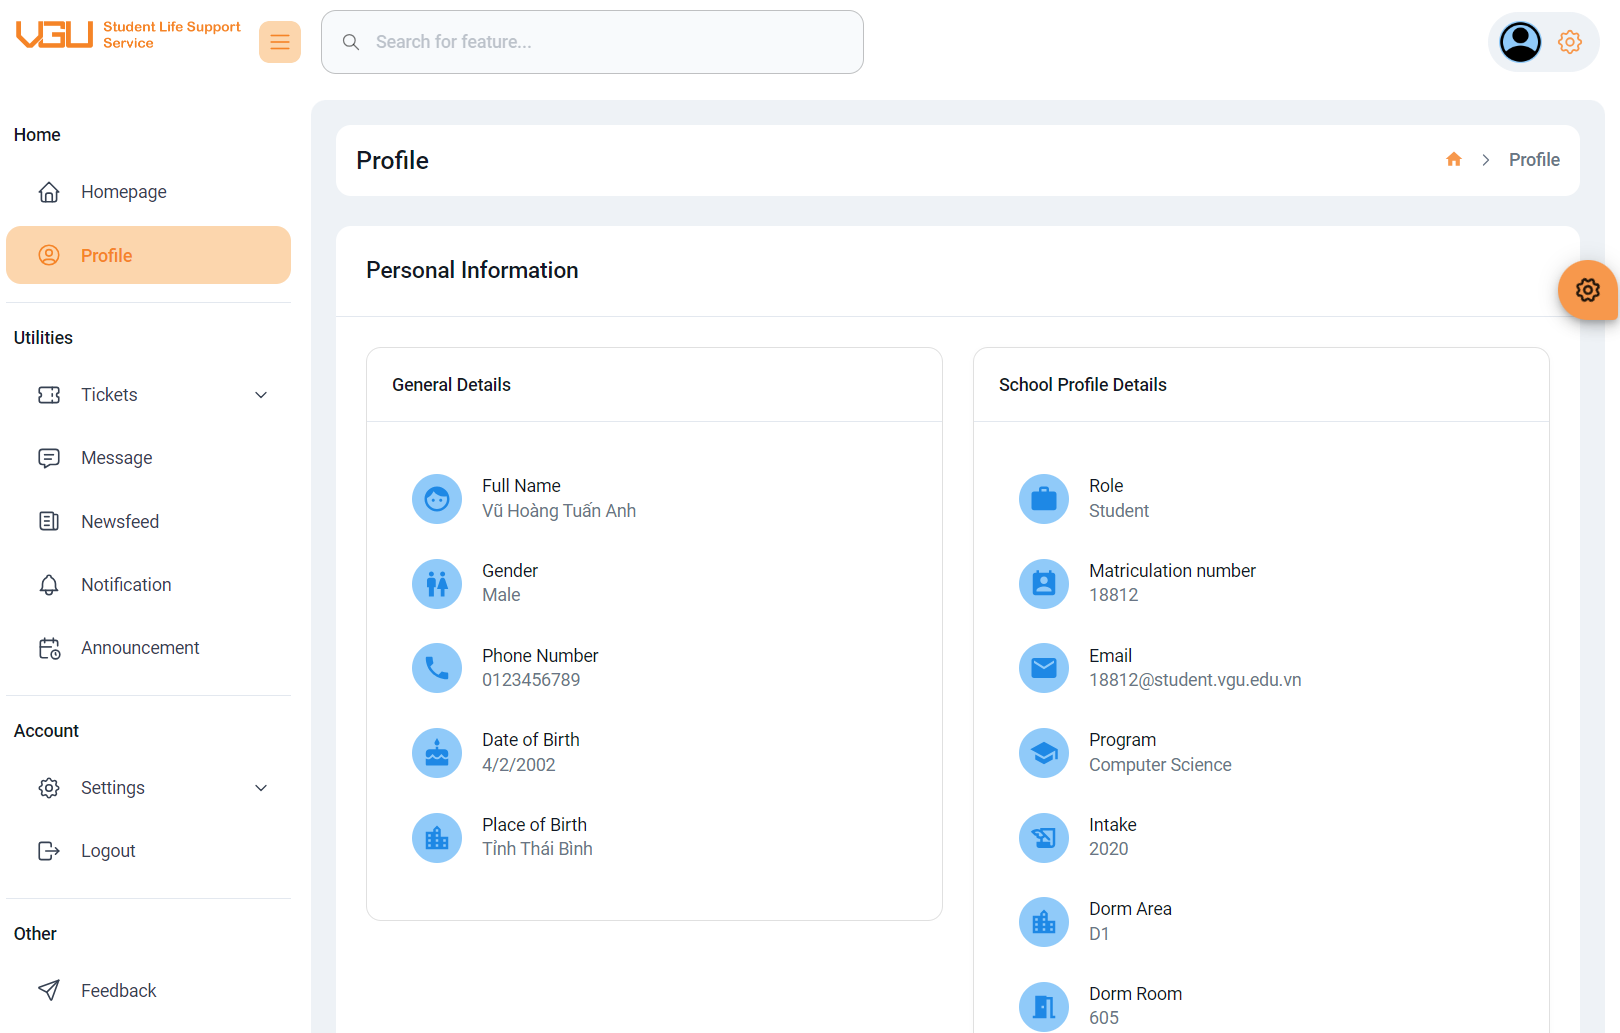
\includegraphics[width=1\linewidth]{graphics/responsive/res2}
		\caption{Profile UI in Desktop device}
		\label{fig:res2}
	\end{figure}
	
	
	\begin{figure}[H]
		\centering
		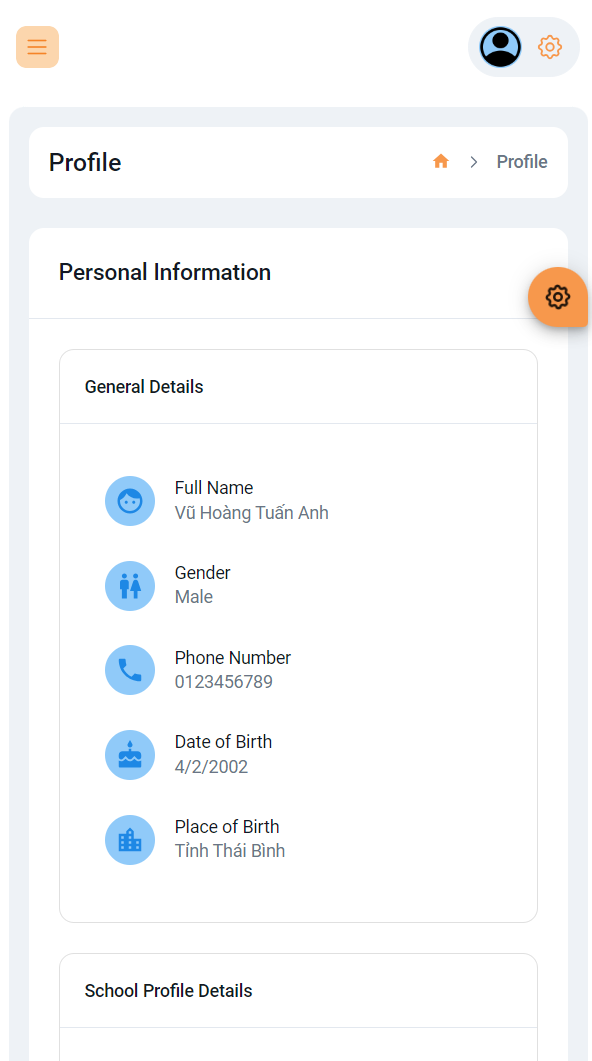
\includegraphics[width=0.5\linewidth]{graphics/responsive/res1}
		\caption{Profile UI in Mobile device}
		\label{fig:res1}
	\end{figure}
	

	
	
	\subsubsection{Live Customization}
	Users have the ability to personalize the web application in real-time by selecting the "Live Customize" option. Within this feature, they can choose from a variety of font families and adjust the border radius to suit their preferences. This functionality not only allows users to create a more tailored and visually appealing experience but also significantly enhances overall user experience (UX). By empowering users to modify these visual elements according to their individual tastes, the application becomes more engaging and user-friendly, ultimately leading to greater satisfaction and a more enjoyable interaction with the platform.
	\begin{figure}[H]
		\centering
		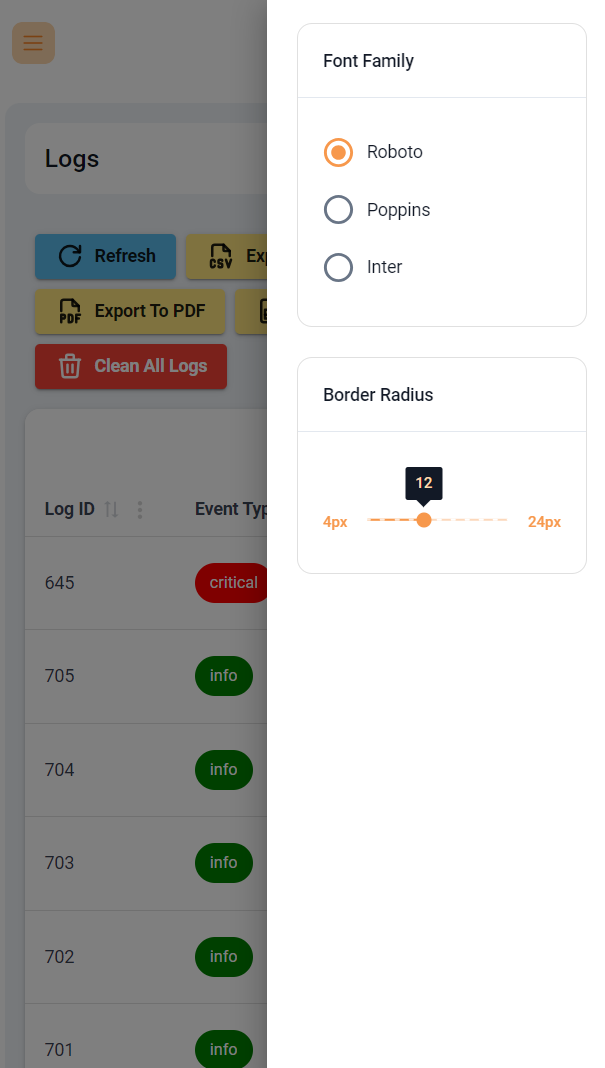
\includegraphics[width=0.5\linewidth]{graphics/responsive/live-custom}
		\caption{Web UI Live Customization}
		\label{fig:live-custom}
	\end{figure}
	
	
	












%	
	


	